\chapter{Specifications}
\label{chapter:specifications}
In this chapter, we describe precisely the IT related specifications (e.g. REST routes, data format, GUI).

%-------------------------------------------------------------------------------
%-------------------------------------------------------------------------------
\section{System architecture}
TODO graphical representation of the system

%-------------------------------------------------------------------------------
%-------------------------------------------------------------------------------
\section{Flow diagram}
The figure~\ref{fig:specs:flowdiagram} defines precisely how the user interacts with the application. It allows to have a clear representation of the system.

\begin{figure}[ht!]
    \centering
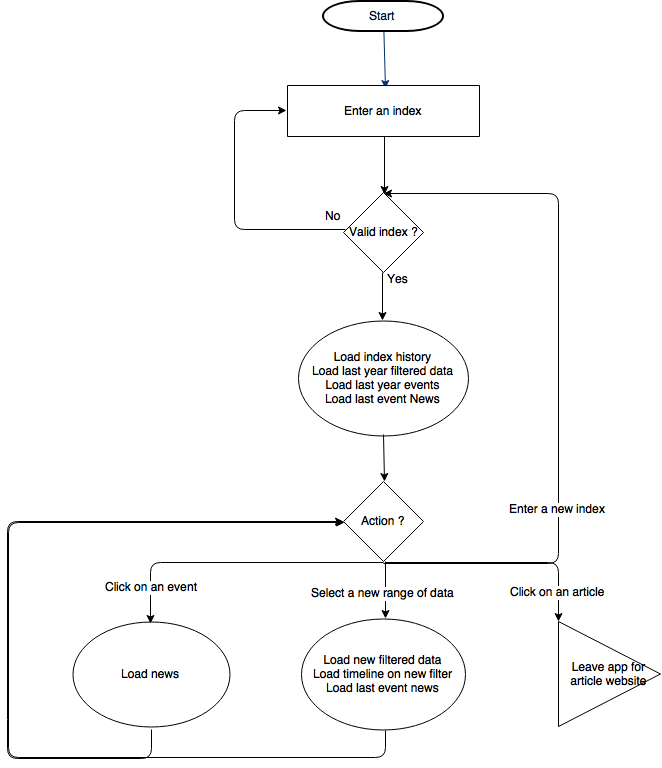
\includegraphics[scale=0.5]{Figures/workflow-stockstrooper.png}
\caption{Flow diagram of the user interaction}
\label{fig:specs:flowdiagram}
\end{figure}

%-------------------------------------------------------------------------------
%-------------------------------------------------------------------------------
\section{REST API}

%-------------------------------------------------------------------------------
\subsection{Routes and format}

\subsubsection*{GET events}
This route sends all events within a period for one index. Default is one year from present.
\begin{verbatim}
/events/:index[/:datestart/:dateend]

[
    {"date": "20160111"},
    {"date": "20160212"},
    {"date": "20160313"}
]
\end{verbatim}

\subsubsection*{GET stocks}
This route sends all the stocks data for one index (market index).
\begin{verbatim}
/stocks/:index

[
    {
        "date": "20160111"
        "value": 14.04
    },
    {
        "date": "20160112"
        "value": 15.04
    },
        "date": "20160113"
        "value": 19.04
    }
]
\end{verbatim}

\subsubsection*{GET news}
This route sends all the news related to one index and one event.
\begin{verbatim}
/news/:index/:dateevent

[
    {
        "headline": "Huge drop for apple",
        "description": "Lorem ipsum dolor sit amet, consectetur
adipiscing elit. Vestibulum laoreet suscipit tristique. Donec
suscipit velit id feugiat placerat. Ut eget egestas risus,
at fermentum ipsum.",
        "date": "20160112",
        "source": "Reuters",
        "url": "http://www.reuters.com/?a=xT6sSPOe99"
    }
]
\end{verbatim}

\subsubsection*{GET index valid}
This route sends a boolean variable which indicates if the index is valid or not.
\begin{verbatim}
/index/:index/

{
    "valid": true
}
\end{verbatim}
%-------------------------------------------------------------------------------
\subsection{CORS}
